\documentclass{article}
\usepackage{blindtext}
\usepackage[a4paper, total={6in, 9.4in}]{geometry}

\usepackage{wrapfig}
\usepackage{graphicx}
\usepackage{mathtext}
\usepackage{amsmath}
\usepackage{siunitx} % Required for alignment
\usepackage{subfigure}
\usepackage{multirow}
\usepackage{rotating}
\usepackage[T1,T2A]{fontenc}
\usepackage[russian]{babel}
\usepackage{caption}
\usepackage{physics}
\usepackage{booktabs}

\graphicspath{{pictures/}}

\title{\begin{center}Лабораторная работа №3.3.5\end{center}
Эффект Холла в металах}
\author{Гёлецян А.Г.}
\date{\today}

\begin{document}

\pagenumbering{gobble}
\maketitle
\newpage
\pagenumbering{arabic}

\textbf{Цель работы:} Измерение подвижности и концентрации носителей заряда в металлах.

\section{Теоретическая часть}
\paragraph{Эффет Холла}
При наличии поперечного магнитного поля в проводнике возникает поперечное напряжение,
которую можно посчитать формулой
\begin{equation}
U_{\perp} = \frac{B}{nqh} \cdot I = R_{H} \cdot \frac{B}{h} \cdot I
\end{equation}
где $h$\textendashтолщина проводящего слоя. Используя связь проводимости (удельного
сопротивления) и подвижности подвижных зарядов получим формулу для подвижности
\begin{equation}
\mu=\frac{1}{nq} \cdot \sigma = \frac{R_{H}}{\rho}
\end{equation}

\section{Ход работы}

\begin{figure}[h]
    \begin{center}
        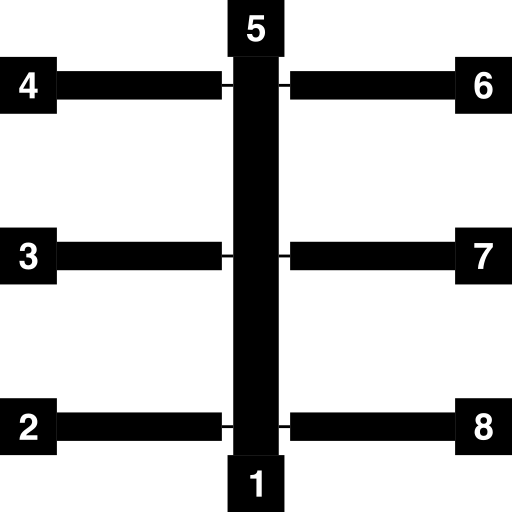
\includegraphics[width=0.3\textwidth]{spider}
    \end{center}
    \caption{Образец из алюминия}
    \label{spider}
\end{figure}

Измерим удельное сопротивления алюминия подключив омметр на контакты $2,3,4,6,7,8$.
Для нашего образца толщина $h=50нм$, ширина $w=0.8мм$,
а расстояние между соседними квадратами $l=1.50мм$.
\begin{equation*}
    \rho = \frac{whR}{L}
\end{equation*}
Проводя измерения получаем

\begin{table}[h]
\begin{center}
\begin{tabular}{c r r}
контакты & $\rho, \Omega \cdot нм$ &  $\Delta \rho, \Omega \cdot нм$ \\\midrule
   2\textendash4 & 36.9 & 0.3 \\
   8\textendash6 & 36.9 & 0.3 \\
   2\textendash3 & 36.9 & 0.6 \\
   3\textendash4 & 36.8 & 0.6 \\
   6\textendash7 & 36.9 & 0.6 \\
   4\textendash7 & 36.8 & 0.6 \\
   7\textendash8 & 36.9 & 0.6 \\
   4\textendash8 & 36.9 & 0.3 \\
\end{tabular}
\caption{Удельное сопротивление материала образца}
\end{center}
\end{table}

Получаем значение
\begin{equation}
    \bar{\rho} = (36.9 \pm 0.3) \Omega \cdot нм
\end{equation}

\newpage

\paragraph{}
Перейдем непосредственно к измерению эффекта Холла
\begin{figure}[h]
    \begin{center}
        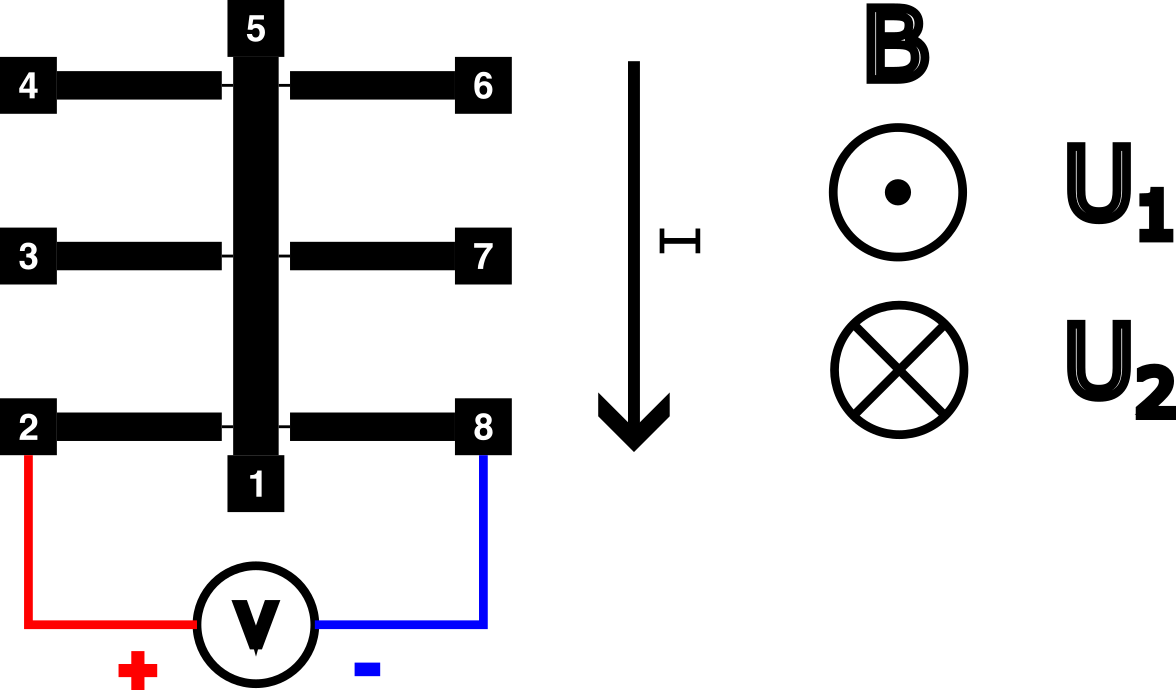
\includegraphics[width=0.5\textwidth]{measurement.png}
    \end{center}
    \caption{Схема измерения}
    \label{measurement}
\end{figure}

Меняя внешнее магнитное поле, а так же силу протекающего тока получим зависимость
$U=U(I, B)$.

\begin{figure}[h]
    \begin{center}
        \includegraphics[width=0.72\textwidth]{plot_IUB.eps}
    \end{center}
    \caption{Схема измерения}
    \label{IUB}
\end{figure}

\newpage

\begin{table}[h]
\begin{center}
\begin{tabular}{rrr rrr rrr}
\toprule
\multicolumn{3}{c}{Контакты 2-8} & \multicolumn{3}{c}{Контакты 3 7} & \multicolumn{3}{c}{Контакты 4-6} \\
$B$  &  $I$   &  $U$     & $B$  &   $I$   &  $U$     & $B$  &   $I$   &  $U$     \\\midrule
508  &  21.12 &  0.00650 & 508  &   20.62 &  0.00655 & 522  &   20.12 &  0.00580 \\
     &  40.60 &  0.01225 &      &   40.57 &  0.01290 &      &   40.49 &  0.01315 \\
     &  60.65 &  0.01895 &      &   60.08 &  0.01865 &      &   60.03 &  0.01835 \\
     &  80.90 &  0.02525 &      &   80.58 &  0.02500 &      &   80.48 &  0.02515 \\
     & 101.05 &  0.03170 &      &  100.84 &  0.03215 &      &  101.09 &  0.03185 \\\midrule
597  &  21.14 &  0.00785 & 593  &   20.62 &  0.00765 & 615  &   20.13 &  0.00785 \\
     &  40.42 &  0.01500 &      &   39.99 &  0.01460 &      &   40.57 &  0.01495 \\
     &  60.00 &  0.02240 &      &   61.36 &  0.02265 &      &   60.67 &  0.02285 \\
     &  79.74 &  0.02995 &      &   80.77 &  0.03005 &      &   80.54 &  0.03025 \\
     & 101.10 &  0.03825 &      &  101.10 &  0.03760 &      &  100.89 &  0.03760 \\\midrule
703  &  20.62 &  0.00905 & 701  &   20.05 &  0.00885 & 708  &   20.26 &  0.00875 \\
     &  39.84 &  0.01755 &      &   40.55 &  0.01760 &      &   40.79 &  0.01745 \\
     &  60.02 &  0.02615 &      &   59.86 &  0.02615 &      &   60.68 &  0.02620 \\
     &  79.84 &  0.03510 &      &   80.46 &  0.03485 &      &   80.58 &  0.03475 \\
     &  99.99 &  0.04405 &      &   99.76 &  0.04385 &      &  100.85 &  0.04285 \\\midrule
840  &  20.60 &  0.01005 & 812  &   20.22 &  0.00980 & 809  &   20.08 &  0.00960 \\
     &  40.05 &  0.01950 &      &   40.55 &  0.01905 &      &   41.06 &  0.01960 \\
     &  60.54 &  0.02975 &      &   59.86 &  0.02915 &      &   60.00 &  0.02830 \\
     &  79.85 &  0.03955 &      &   80.46 &  0.03910 &      &   80.94 &  0.03835 \\
     &  99.99 &  0.04940 &      &   99.76 &  0.04860 &      &  100.40 &  0.04760 \\\midrule
923  &  20.85 &  0.01070 & 909  &   20.70 &  0.01075 & 906  &   20.60 &  0.01070 \\
     &  40.02 &  0.02070 &      &   40.59 &  0.02100 &      &   40.31 &  0.02040 \\
     &  60.72 &  0.03160 &      &   60.70 &  0.03135 &      &   60.69 &  0.03070 \\
     &  81.42 &  0.04295 &      &   79.69 &  0.04140 &      &   81.44 &  0.04085 \\
     & 101.10 &  0.05325 &      &  101.43 &  0.05255 &      &  100.93 &  0.05170 \\\midrule
1031 &  21.10 &  0.01185 & 1033 &   20.33 &  0.01150 & 991  &   20.23 &  0.01120 \\
     &  40.62 &  0.02280 &      &   40.61 &  0.02280 &      &   40.84 &  0.02175 \\
     &  60.08 &  0.03365 &      &   60.72 &  0.03470 &      &   60.11 &  0.03265 \\
     &  81.45 &  0.04610 &      &   80.43 &  0.04575 &      &   80.58 &  0.04330 \\
     &  99.99 &  0.05650 &      &  100.95 &  0.05715 &      &  100.72 &  0.05475 \\\bottomrule
\end{tabular}
\caption{Данные измерении в единицах $(мТ, мА, мВ)$}
\end{center}
\end{table}
\newpage

\paragraph{}
Согласно формуле (1)
\begin{equation}
    Uh = (IB) \cdot R_H
\end{equation}
Исследуем зависимость $y=y(x)$ где $y=Uh$, $x=IB$. Она должна быль линейной с 
коэффицентом наклона равной $R_H$. Заметим что из знака $U$ и направления 
магнитного поля можно сделать вывод что в алюмине носителями заряда являются электроны,
следовательно $R_H < 0$

\begin{figure}[h]
    \begin{center}
        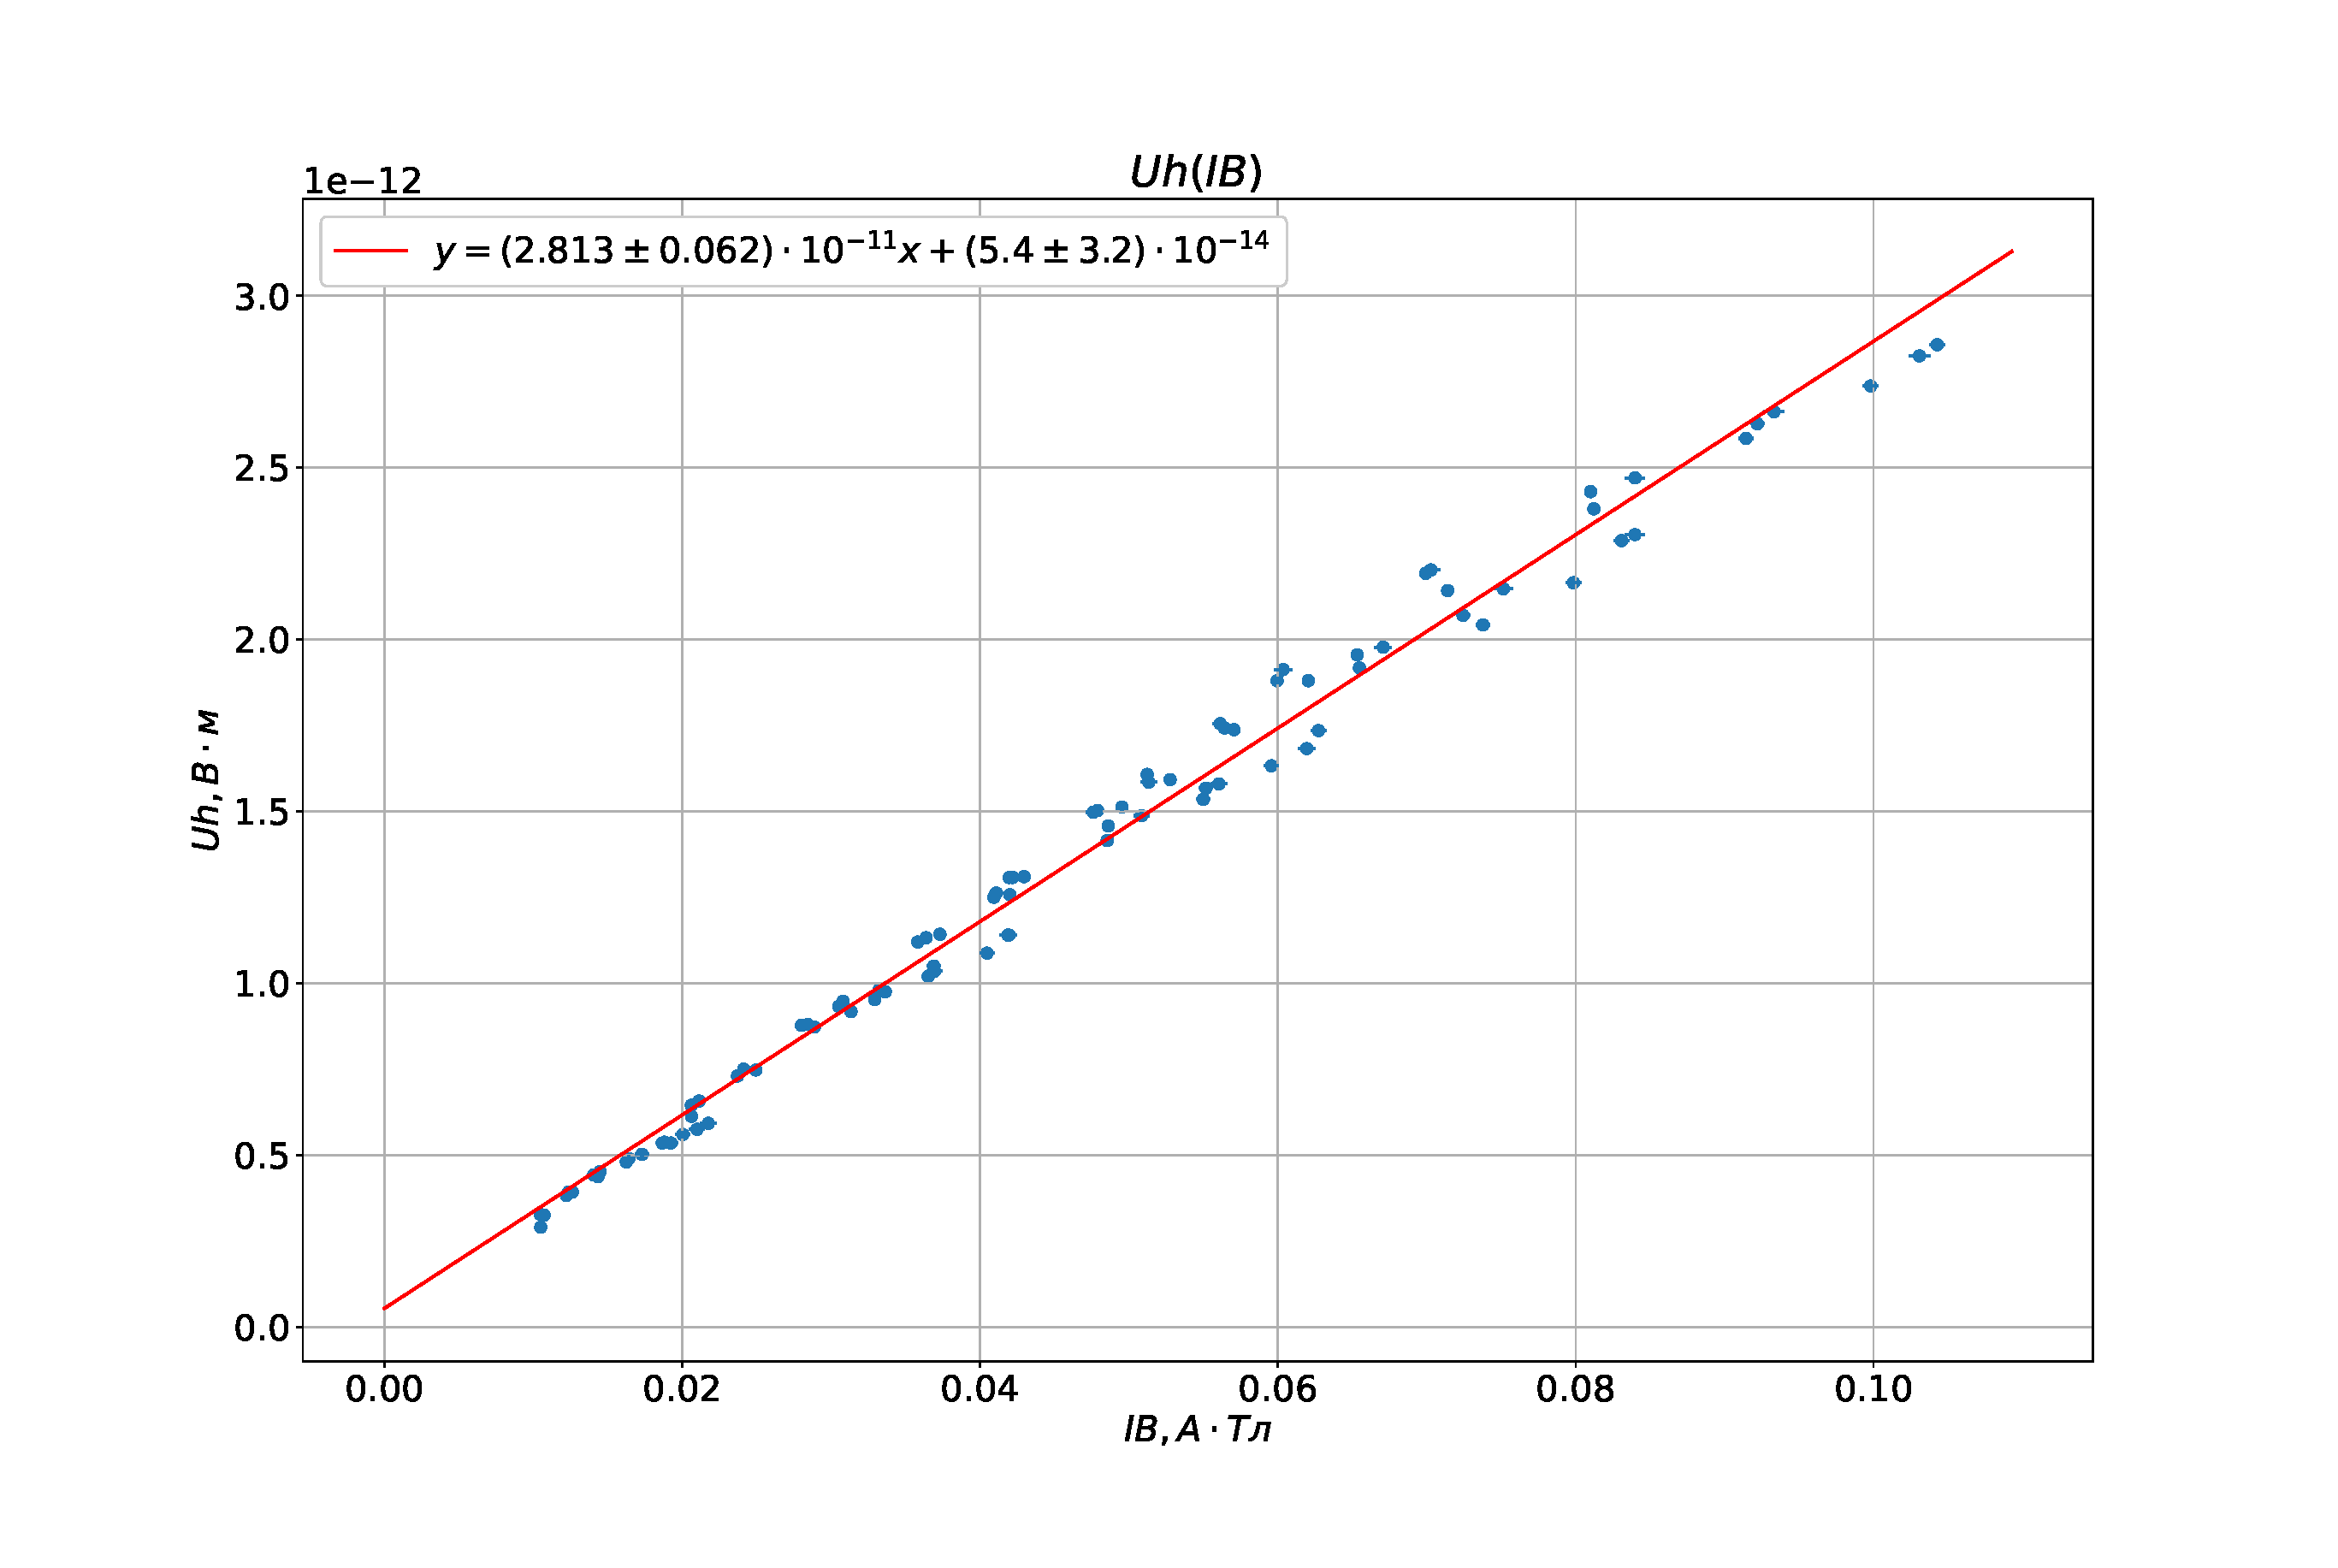
\includegraphics[width=1\textwidth]{plot.eps}
    \end{center}
    \caption{Определение постоянной Холла}
\label{plit}
\end{figure}

Получаем значение
\begin{equation}
    R_H = -(2.813 \pm 0.062) \cdot 10^{-11} м^3 Кл^{-1}
\end{equation}
Отсюда высчитываем концентрацию свободных электронов и их подвижность
\begin{equation}
    n = \frac{-1}{R_H e} = (2.22 \pm 0.05) \cdot 10^{29} м^{-3}
\end{equation}
\begin{equation}
    \mu=\frac{R_{H}}{\rho}=(7.62 \pm 0.18) \cdot 10^{-4} м^2В^{-1}с^{-1}
\end{equation}

\section{Выводы}
Для чистого алюминия имеем следующие данные
\begin{equation}
    \rho_{таб}=26.3 \Omega \cdot нм \text{,  }
    R_{H,таб}=-3.4 \cdot 10^{-11}м^{3}Кл^{-1} \text{,  }
    \mu_{таб}=13\cdot 10^{-4}м^{2}В^{-1}с^{-1}
\end{equation}
Как видим наши значения не совпадают с табличными значеняими, что скорее всего связано
наличием примесей в нашем образце.

\end{document}

